\documentclass{memoria}
\usepackage{algorithm}
\usepackage{algpseudocode}
\usepackage{float}
\usepackage{multirow}
\usepackage{graphicx}
\usepackage{subcaption}
\usepackage{hyperref}
\usepackage{adjustbox}
\setcounter{secnumdepth}{4}
\usepackage[table,xcdraw]{xcolor}

\algdef{SE}[VARIABLES]{Variables}{EndVariables}
   {\algorithmicvariables}
   {\algorithmicend\ \algorithmicvariables}
\algnewcommand{\algorithmicvariables}{\textbf{global variables}}

\begin{document}
\pagestyle{empty} % retira numeracion de paginas
%datos%
\author{Luis González Romero, XXXXXXXXX, luisgonromero@correo.ugr.es}
\title{Práctica 3: Implementación distribuida de un algoritmo de equilibrado dinámco de la carga usando MPI. TSP con Branch\&Bound}
\newcommand{\grupopracticas}{Grupo 1: Miércoles 09:30-11:30}
\newcommand{\subtitulo}{Subtítulo}
\newcommand{\curso}{Programación Paralela}
\newcommand{\departamento}{Lenguajes y Sistemas Informáticos}

\begin{center}
\LARGE{\bf \thetitle:}\\
%\Large{\bf \subtitulo}\\
\end{center}

%\vspace{1em}


%\vfill


\begin{figure}[H]
\centering

\includegraphics[scale=0.8]{imagenes/logo.png}
\end{figure}


\begin{center}
\theauthor
\\
%\grupopracticas
\end{center}

\begin{center}
Escuela Técnica Superior de Ingeniería informática y Telecomunicaciones

\end{center}

%\vspace{2in}

\begin{center}
\today
%\displaydate{date}
\end{center}
%\afterpage{\blankpage \addtocounter{page}{1}} %addtocounter incrementa numero de pagina ya que blankpage no lo hace%



%Lista de figuras%
%\renewcommand{\listfigurename}{\centering LISTA DE FIGURAS}
%\listoffigures
%\newpage

%Lista de tabelas%
%\renewcommand{\listtablename}{\centering Índice de tablas}
%\listoftables
%\newpage

%Sumario%

\newpage
\section{Transformación vectorial iterativa}

\begin{figure}[H]
\centering
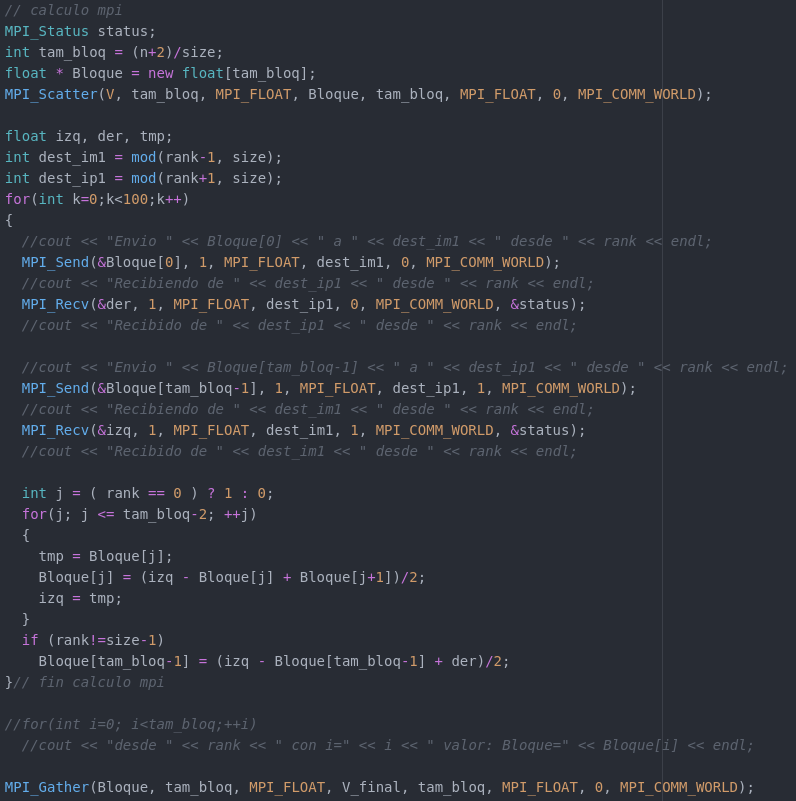
\includegraphics[width=0.8\textwidth]{imagenes/code.png}
\end{figure}

Cada proceso tiene un tamaño de bloque igual a una parte igual de $n$ más los dos extremos. Se envía casi de forma idéntica que en el pseudocódigo mostrado en las transparencias y se calcula igual excepto para los extremos: rank(0) no ejecuta la iteración 0 y rank(size-1) no ejecuta la ultima.

Finalmente se hace el gather de todos los bloques. A continuación se muestra una ejecución para n=12(10+2), en la que se pasa el mismo test que en las prácticas y se muestran todos los elementos de los vectores.

\begin{figure}[H]
\centering
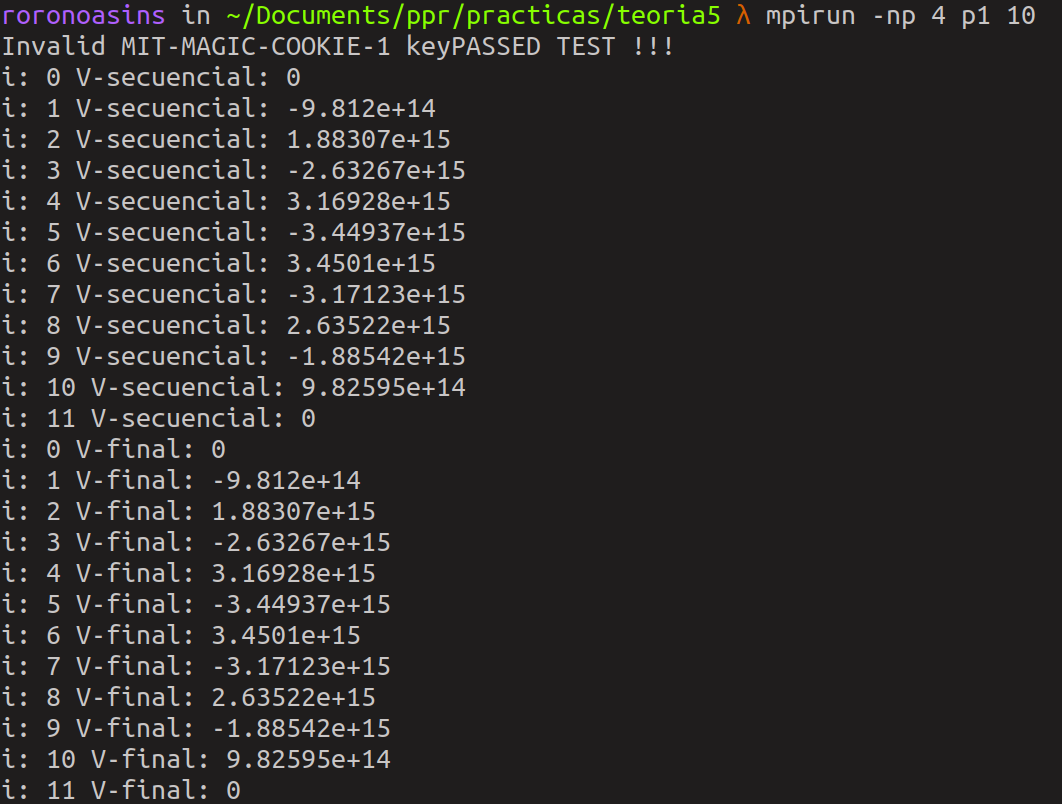
\includegraphics[width=0.8\textwidth]{imagenes/ej.png}
\end{figure}


%\input{2}
%\input{3}


%%%%%%%%%%%%%%%%%%%%%%%%%%%%% Referencias %%%%%%%%%%%%%%%%%%%%%%%%%%%%%
%\renewcommand{\refname}{\centering REFERENCIAS} %Centrar%
%\addcontentsline{toc}{section}{Referencias} % añade referencias al indice

\nocite{*}
\bibliographystyle{unsrt}
%\bibliography{references}


\end{document}